
\documentclass[12pt]{ctexart}

\usepackage{graphicx}
\usepackage{amsmath}
\usepackage{booktabs}

\title{数学建模环境测试}
\author{Jack}
\date{\today}

\begin{document}

\maketitle

\section{环境测试}

这是我的第一份 \LaTeX{} 文档

我们已经完成 Python 数据处理、绘图以及结果导出。

\section{简单公式}

例如，平均值可以表示为

\[
\bar{x}
=
\frac{1}{n}
\sum_{i=1}^{n} x_i.
\]

\section{数据可视化}

图~\ref{fig:score} 展示了学生的平均成绩

\begin{figure}[htbp]
    \centering
    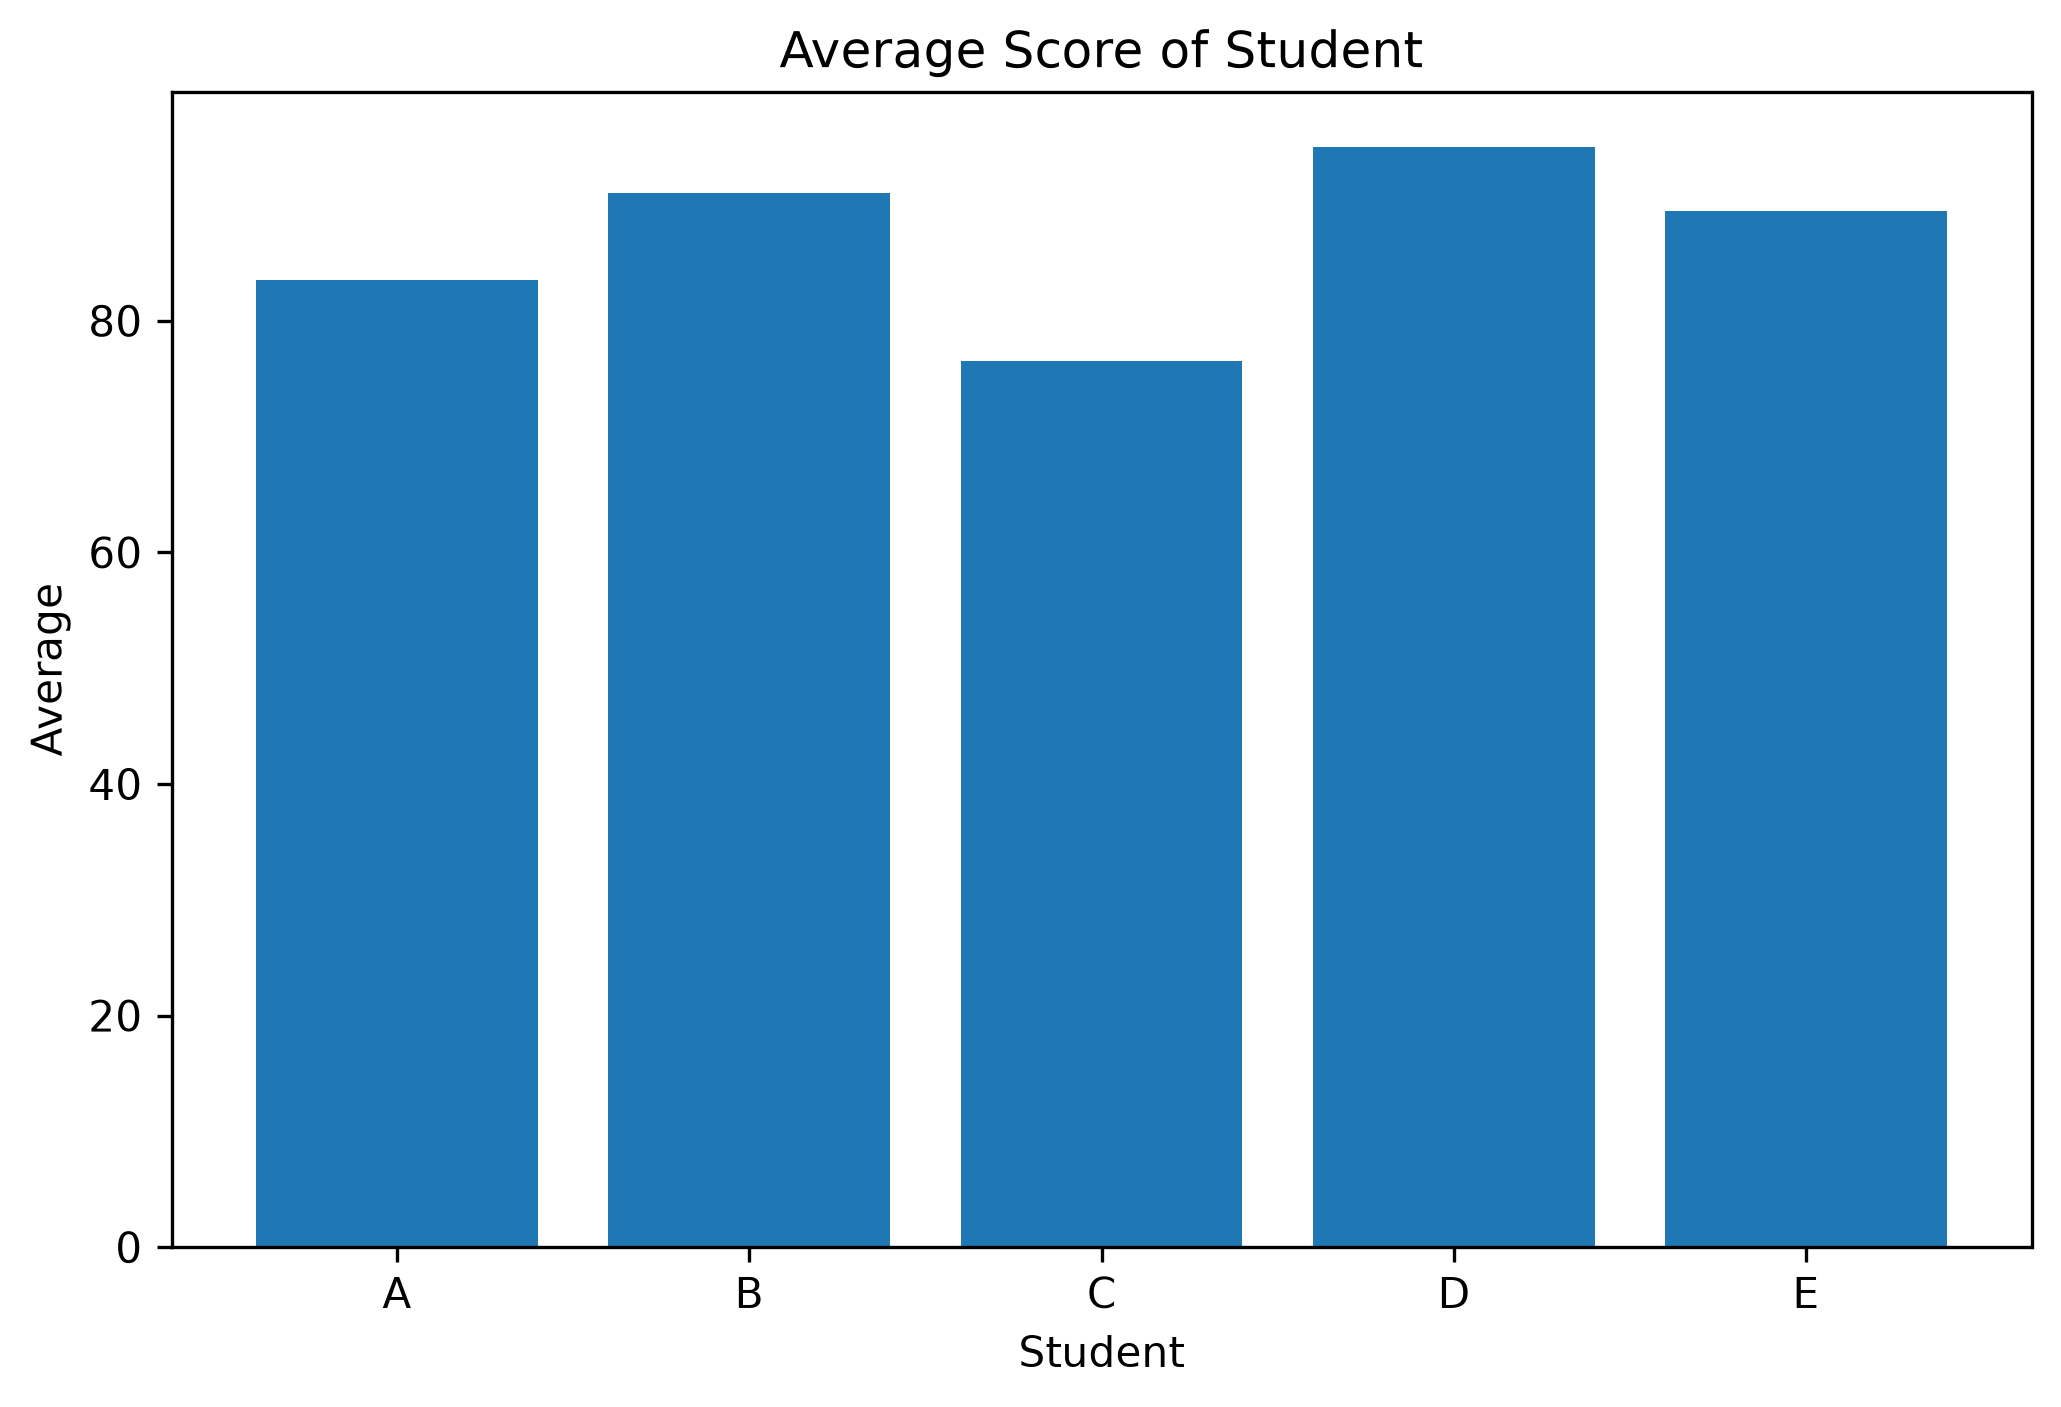
\includegraphics[width = 0.75\textwidth]
    {../figures/test_plot.png}
    \caption{学生平均成绩}
    \label{fig:score}
\end{figure}

\section{结果表格}

\begin{table}[htbp]
    \centering
    \caption{学生成绩实例}
    \begin{tabular}{cccc}
        \toprule
        学生 & 数学 & 物理 & 平均分 \\
        \midrule
        A & 85 & 82 & 83.5 \\
        B & 92 & 90 & 91.0 \\
        C & 78 & 75 & 76.5 \\
        D & 96 & 94 & 95.0 \\
        E & 88 & 91 & 89.5 \\
        \bottomrule
    \end{tabular}
\end{table}

\end{document}